\documentclass[12pt,a4paper]{ctexart}
\usepackage[utf8]{inputenc}
\usepackage{amsmath}
\usepackage{amsfonts}
\usepackage{amssymb}
\usepackage{graphicx}
\usepackage{bm}
\usepackage{booktabs}
\usepackage{draftwatermark}
\usepackage[backend=biber,backref=true%nature,% citestyle=gb7714−2015,backref=true%
]{biblatex}
%参考文献数据源加载 
\addbibresource[location=local]{ref.bib}
\usepackage[table,xcdraw]{xcolor}
\usepackage{float}
%\usepackage[left=3.0cm, right=3.0cm, top=3.5cm, bottom=2.70cm]{geometry}
\title{隐马尔科夫模型 \\
	在拼音输入法中的应用研究}
\author{Yuan}
\date{\small\today}
\begin{document}

\maketitle
\begin{abstract}
本文尝试将隐马尔科夫模型应用于中文整句拼音输入法,给出了具体的模型和实际问题的对应关系以及参数估计的方法。同时还选用了现有的中文语料库进行了实验验证,取得了较好的效果。
\end{abstract}	
\section{引言}
隐马尔科夫模型(Hidden Markov Model,HMM)是一种应用于序列问题的统计学系模型,该模型描述了由隐藏的马尔科夫链随机生成观测序列的过程。HMM非常适合解决标注问题,故HMM在语音识别、自然语言处理、生物信息、模式识别等领域有广泛的\cite{李航统计学习},本文着眼于将HMM应用于中文拼音输入法。拼音输入法将拼音转换为对应汉字,其中更具有实用价值的是将连续的拼音输入转换为连续的句子。这是典型的序列问题,更为具体地,是一种序列标注问题,故应用HMM能较好的解决该问题。
\section{问题描述}
HMM描述了一个隐藏的马尔科夫链生成不可观测的状态随机序列,再由各个状态生成一个观测而产生观测随机序列的过程。HMM随机生成的状态序列成为状态序列(state sequence);每一个状态生成一个观测,而由此产生的观测的随机序列成为观测序列(observation sequence)。故HMM可以由初始概率分布、状态转移概率分布以及观测概率分布确定,这三者对应的参数分别为初始状态概率向量$ \bm{\pi} $、状态转移概率矩阵$\bm{A}$及观测概率矩阵$\bm{B}$。由此HMM可以用三元组$ \lambda=(\bm{A},\bm{B},\bm{\pi}) $表示\cite{李航统计学习}。

在拼音序列转汉字的问题中,连续的句子被视为序列,即认为每个时刻对应一个汉字,汉字又对应拼音。由于用户在输入法中输入的是拼音,所以拼音序列被定义为观测序列。而汉字则为生成观测序列的状态序列。要解决通过观测序列得到最有可能的状态序列实质是求解一个最大路径问题,Viterbi算法\cite{viterbi2006a}被用于解决该问题。
\subsection{模型定义}
对于拼音序列转汉字问题的的HMM相关定义如下:


所有的汉字组成集合Q(状态集合),所有汉字对应的拼音的集合V(观测集合),其中$ |Q|=N, |V|=M $。
\[ Q=\{ \mbox{汉字}_1,\mbox{汉字}_2,\cdots,\mbox{汉字}_N \},V=\{ \mbox{拼音}_1,\mbox{拼音}_2,\cdots,\mbox{拼音}_M \}  \]

用户想输入的汉字序列I(状态序列),用户实际输入的拼音序列O(观测序列),其中$ |I|=|O|=T $。
\[ I=\{ \mbox{预期汉字}_1,\mbox{预期汉字}_2,\cdots,\mbox{预期汉字}_T \}	\]
\[O=\{ \mbox{输入拼音}_1,\mbox{输入拼音}_2,\cdots,\mbox{输入拼音}_T \}  \]

句子中前后汉字转移概率矩阵$\bm{A}$:
\[ \bm{A}=[a_{ij}]_{N\times N} \]
其中,
\[ a_{ij}=P(i_{t+1}=\mbox{汉字}_j|i_t=\mbox{汉字}_i),  i=1,2,3,\cdots,N; j=1,2,\cdots,N\]
是在句子中的位置$ t $处的$ \mbox{汉字}_i $转移到$ t+1 $处的$ \mbox{汉字}_j $的概率。
句子中前后汉字转移概率矩阵$\bm{B}$:
\[ \bm{B}=[b_j(k)]_{N\times M} \]
其中,
\[ b_j(k)=P(\mbox{第t个输入的拼音}=\mbox{拼音}_k|\mbox{第t个想要输入的汉字}=\mbox{汉字}_j) \]
\[ k=1,2,3,\cdots,M; j=1,2,\cdots,N\]
是在句子中的位置$ t $处的$ \mbox{汉字}_j $生成$ \mbox{拼音}_k $的概率。

句子中首个汉字出现可能性的概率向量$\bm{\pi}$:
\[ \bm{\pi}=(\pi_i) \]
其中,
\[ \pi_i=P(\mbox{句首汉字}=\mbox{汉字}_i), i=1,2,\cdots,N \]
是句首汉字为$\mbox{汉字}_i$的概率。
\subsection{模型训练(参数估计)}
HMM的训练可以采用监督学习或者无监督学习\cite{李航统计学习},本应用的状态和观测为汉字和拼音。将汉字转化为拼音可以自动开展\cite{python-pinyin},并有相当高的准确度\cite{accuracy-of-auto-pinyin}。故可以通过中文语料库生成用于监督学习的训练集。
本应用中HMM的三元组$ \lambda=(\bm{A},\bm{B},\bm{\pi}) $的估计方法如下:
\paragraph{前后汉字转移概率$a_{ij}$的估计}
设句子中第$ t $个$\mbox{汉字}_i$转移到第$ t+1 $个的$\mbox{汉字}_j$的频数为$A_{ij}$,状态转移概率$a_{ij}$的估计是:
\[ \hat{a}_{i j}=\frac{A_{ij}}{\sum_{j=1}^{N} A_{i j}}, \quad i=1,2, \cdots, N ; j=1,2, \cdots, N \]
\paragraph{汉字转拼音的概率$b_j(k)$的估计}
设句子中$\mbox{汉字}_j$被观测为$\mbox{拼音}_k$的频数是$B_{j k}$,那么$\mbox{汉字}_j$观测为$\mbox{拼音}_k$的概率$b_{j}(k)$的估计是:
\[ \hat{b}_{j}(k)=\frac{B_{j k}}{\sum_{k=1}^{M} B_{j k}}, \quad j=1,2, \cdots, N ; k=1,2, \cdots, M \]
\paragraph{句首汉字出现概率$\pi_i$的估计}
初始状态概率$\pi_i$的估计$\hat{\pi}_i$为S个句子样本中句首汉字为$\mbox{汉字}_i$的频率。


\section{实验}
\subsection{数据集来源及处理}
参数估计使用的语料源自搜狗实验室提供的搜狐往年的新闻数据集\cite{SogouCS}。原始的数据集非常庞大,通过清洗整理后得到如表\ref{table:dataset-stat}所述的数据集,其中的最大值、最小值、均值及方差是基于句子长度统计的;图\ref{fig:datasethistogram}给出了具体的句子长度频率分布,可以发现大部分样本的长度集中在30以内。这些数据集的句子同时使用文字转拼音的自动化程序\cite{python-pinyin}产生对应的拼音。训练集和测试集选自原数据集的不同位置,没有交集。
\bigskip
\begin{figure}[H]
	\centering
	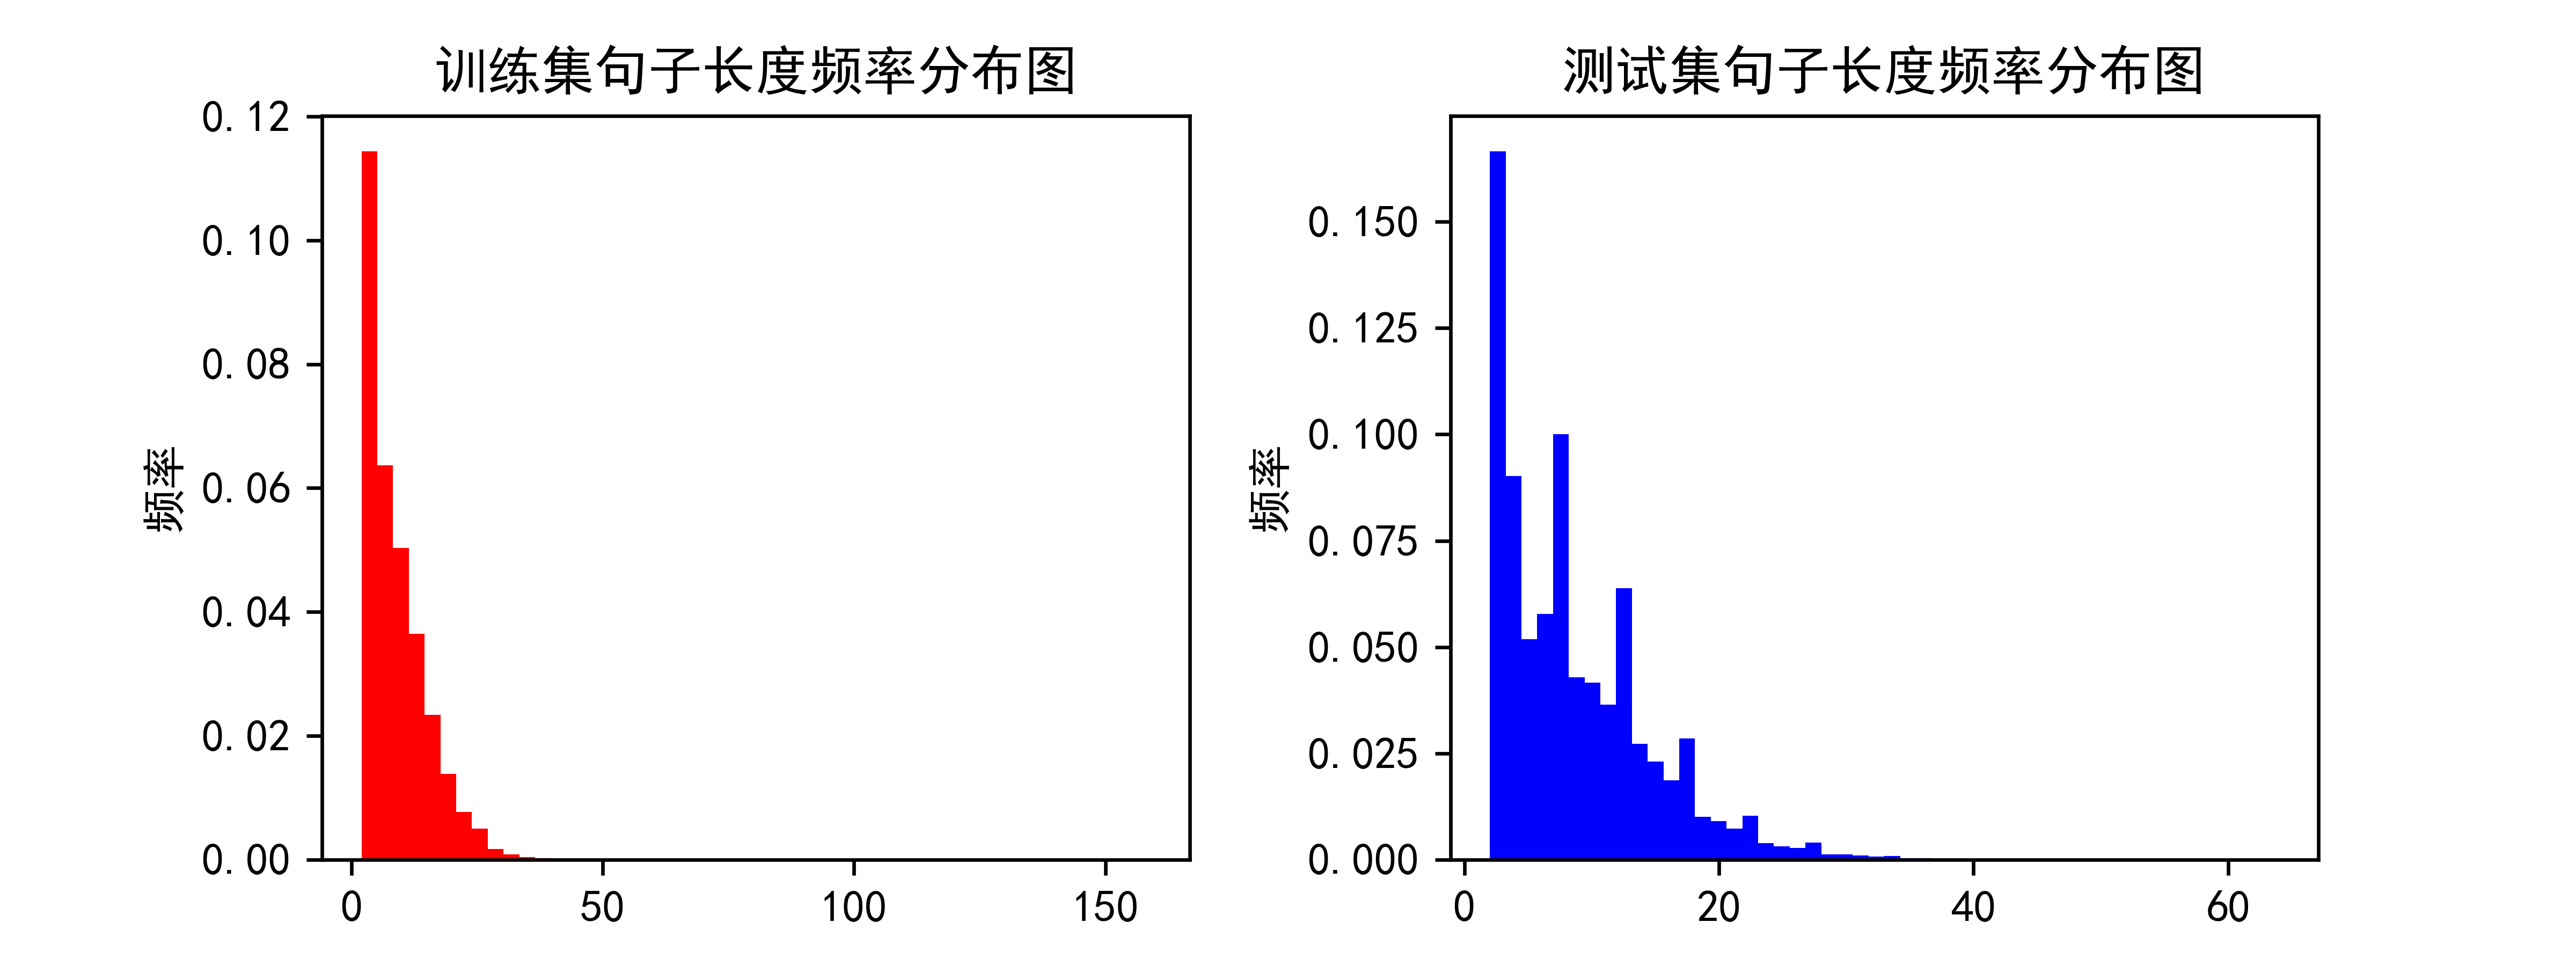
\includegraphics[width=1\linewidth]{DataSetHistogram}
	\caption{数据集句子长度分布}
	\label{fig:datasethistogram}
\end{figure}
\bigskip
\begin{table}[H]
	\centering
\begin{tabular}{cccccc}
	\toprule  %添加表格头部粗线
	数据集 & 样本数 & 最大值 & 最小值& 均值& 标准差\\
	\midrule  %添加表格中横线
		训练集 & 8000000       & 159 & 2&8.91 & 6.09\\
测试集 & 100000 & 64 & 2 & 8.65 & 6.06\\
	\bottomrule %添加表格底部粗线
\end{tabular}
\caption{实验数据集统计信息}
\label{table:dataset-stat}
\end{table}
\clearpage
\subsection{实验流程及结果}
实验先使用训练集对HMM的参数进行估计,再使用测试集的数据进行测试,即使用测试集的拼音序列作为输入,用HMM给出预测的汉字序列并和测试集对应的序列做比较并量化差异。差异的量化定义为:
\bigskip
\[ \mbox{错误率}=\frac{\mbox{测试序列和预测序列不同的个数}}{\mbox{序列总长度}} \times 100\% \]

\bigskip

实验结果如表\ref{table:experiment-result}所示,其中根据不同长度的句子的结果进行了分组,这是因为考虑到输入法的日常应用场景,低于十个汉字的输入是最频繁的,所以对应的实验结果更具有实际意义。可以发现小于十个汉字的平均错误率在30\%上下,是一个较好的结果,具有使用价值。当句子长度大于10以后错误率也并未提高很多,这得益于选用的数据集数据量较大,即便是本来分布就比较少的长句子也能有足够的样本进行训练。
表\ref{table:prediction-samples}给出了从实验结果中随机抽取的序列,可以发现整体表现还是可以接受。
\bigskip
\bigskip

\begin{table}[H]
	\centering
	\begin{tabular}{@{}ll@{}}
		\toprule
		句子长度 & 平均错误率 \\ \midrule
		任意长度 & 29.7\% \\
		\textless{}=5 & 22.4\% \\
		\textgreater{}5 且 \textless{}=10 & 31.0\% \\
		\textless{}11 且 \textless{}=20 & 36.2\% \\
		\textgreater{}20 & 42.6\% \\ \bottomrule
	\end{tabular}
	\caption{实验结果}
	\label{table:experiment-result}
\end{table}



\clearpage
\begin{table}[H]
	\centering
	\begin{tabular}{@{}ll@{}}
		\toprule
		句子长度                              & 样例                                                                                                                                                                                                                                                          \\ \midrule
		\textless{}=5                     & \begin{tabular}[c]{@{}l@{}}真值:他山之石\\ 预测:他山之时\\真值:政策热\\ 预测:政策热\\真值:还差\\ 预测:还差\end{tabular}                                                                                                                                                           \\ \midrule
		\textgreater{}5 且 \textless{}=10  & \begin{tabular}[c]{@{}l@{}}真值:经顺义法院调解\\ 预测:景顺义法院调解\\真值:自然难免网民说三道四\\ 预测:自然难免网民说三道四\\真值:餐饮的准入条件和标准\\ 预测:餐饮的准入条件和标准\end{tabular}                                                                                                                       \\ \midrule
		\textgreater{}10 且 \textless{}=20 & \begin{tabular}[c]{@{}l@{}}真值:希望可以在我骑行的途中\\ 预测:希望可以在我其行的土重\\真值:这架飞机遭击中时处于国际空域\\ 预测:折价飞机遭击中石出于国际控预\\真值:但民营企业中的大型企业只有\\ 预测:但民营企业中的大型企业之忧\end{tabular}                                                                                                 \\ \midrule
		\textgreater{}20                  & \begin{tabular}[c]{@{}l@{}}真值:所以出国语言类考试的辅导课程也要及时开始涉及\\ 预测:所以出国与研类考试的服到可乘也要集市开始设计\\真值:这种作风也使贾康在公共财政和基层财政改革等方\\             面颇有建树\\ 预测:这种做风也是加抗灾工工采政和技层采政改革等方\\             面破有建树\\真值:地区争端多发和国际恐怖主义横行等多种内外危机\\ 预测:地区政短多发和国际控不住一横行等多种内外围及\end{tabular} \\ \bottomrule
	\end{tabular}
	\caption{预测及真值样例}
	\label{table:prediction-samples}
\end{table}
\clearpage

\section{总结及展望}
本文使用了HMM模型建模了拼音序列转汉字序列的标注问题,给出了具体的实验方案并开展了实验,得到近30\%错误率的表现,具有很高的实用价值。模型还有很大的改进空间,例如在HMM中可的状态序列可以用二阶马尔科夫链描述,相对于只考虑前后关系的一阶马尔科夫链会有更好的表现。


\printbibliography[heading=bibliography,title=参考文献]
\end{document}